
\documentclass{beamer}
\usepackage[latin1]{inputenc}
%\usetheme{Montpellier}
\usetheme{Boadilla}
%\usecolortheme[RGB={204,51,255}]{structure}
%\usecolortheme[named=purple]{structure}
\usecolortheme[RGB={62,128,62}]{structure}
%\definecolor{dark}{rgb}{0.3,0.15,0.3}
%\definecolor{light}{rgb}{0.8,0.6,0.8}
%\definecolor{reddish}{rgb}{.5,0.15,0.15}
\definecolor{dark}{rgb}{0.5,0.3,0.4}
%\definecolor{light}{rgb}{0.8,0.6,0.8}
\definecolor{reddish}{rgb}{.7,0.25,0.25}
\definecolor{greenish}{rgb}{.25,0.7,0.25}
\definecolor{blueish}{rgb}{.25,0.25,0.7}
\definecolor{purple}{rgb}{.5,0.0,0.5}
\usepackage{graphicx}
\usepackage{pstricks}

\newcommand{\crish}{\color{reddish}}
\newcommand{\cbla}{\color{black}}
\newcommand{\cred}{\color{red}}
\newcommand{\cblu}{\color{blue}}

\usepackage{tikz}
\usetikzlibrary{arrows,decorations.markings,positioning}
\usepackage{epstopdf}

\title[Computational Neuroscience 1.1]{Computational Neuroscience 1.1}
\author{PHPH20007}
\institute{\texttt{github.com/conorhoughton/PHPH20007}}
\date{May 2019}

\begin{document}

\maketitle

\begin{frame}{The leaky integrate and fire model}
\color{black}
\color{reddish}
$$
\tau \frac{dV}{dt}=E_l-V+R_mI_e
$$
\color{black}
\end{frame}

\begin{frame}{A leaky bucket}

  \begin{center}
    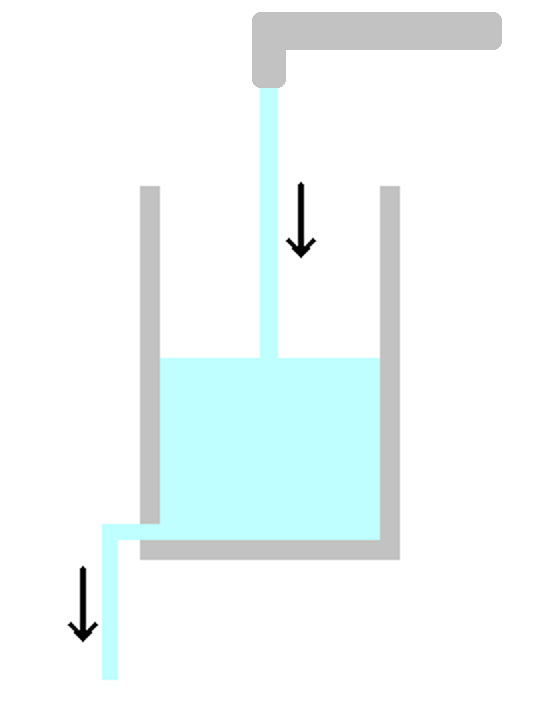
\includegraphics[height=6cm]{glass.png}
  \end{center}
  
  
\end{frame}



\begin{frame}{A leaky bucket}

  \begin{center}
    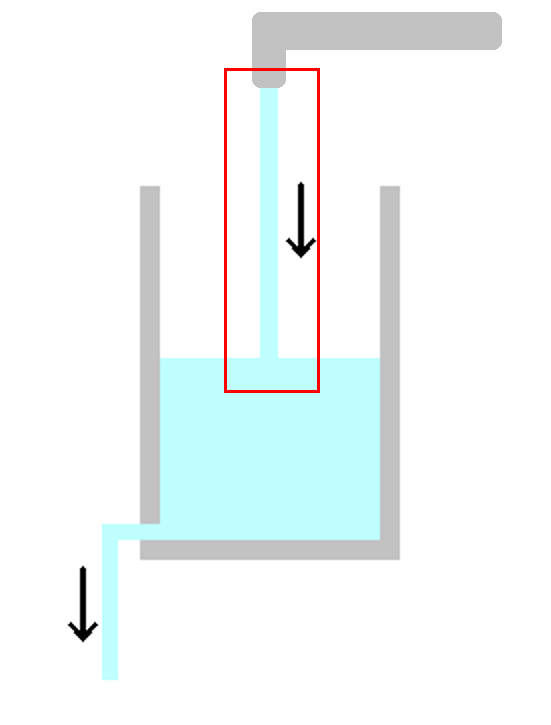
\includegraphics[height=6cm]{glass_in.png}
  \end{center}
  
  
\end{frame}

\begin{frame}{A leaky bucket}

  \begin{center}
    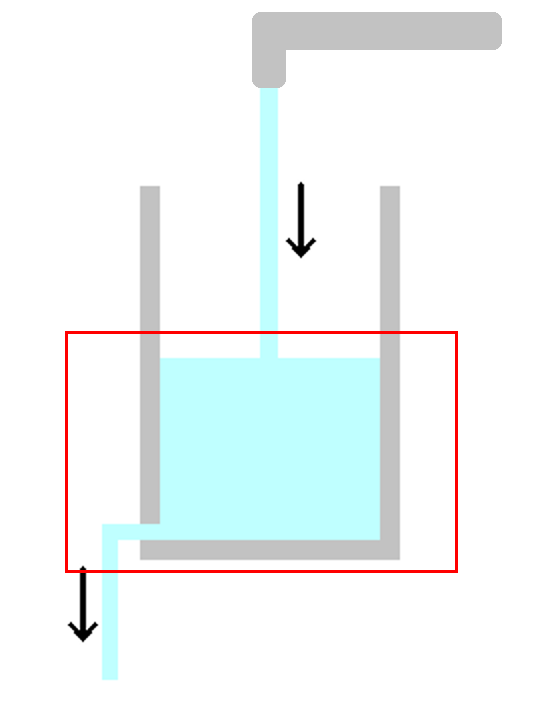
\includegraphics[height=6cm]{glass_contents.png}
  \end{center}
  
  
\end{frame}

\begin{frame}{A leaky bucket}

  \begin{center}
    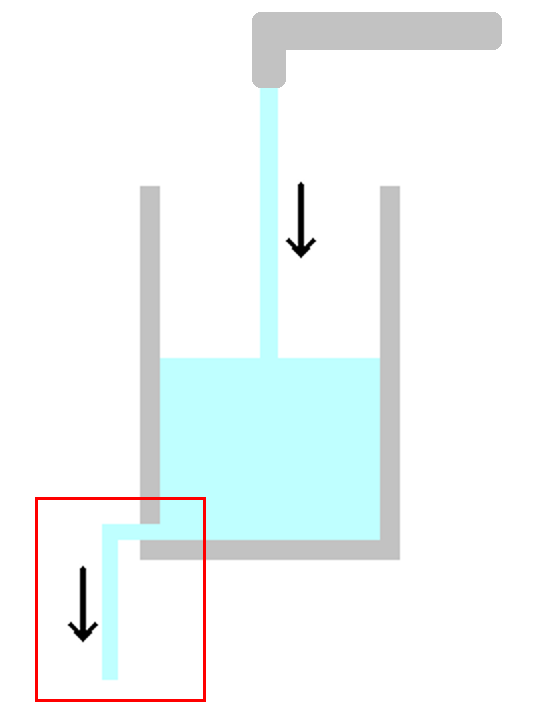
\includegraphics[height=6cm]{glass_out.png}
  \end{center}
  
  
\end{frame}


\begin{frame}{A leaky bucket - increased inflow}

  \begin{center}
    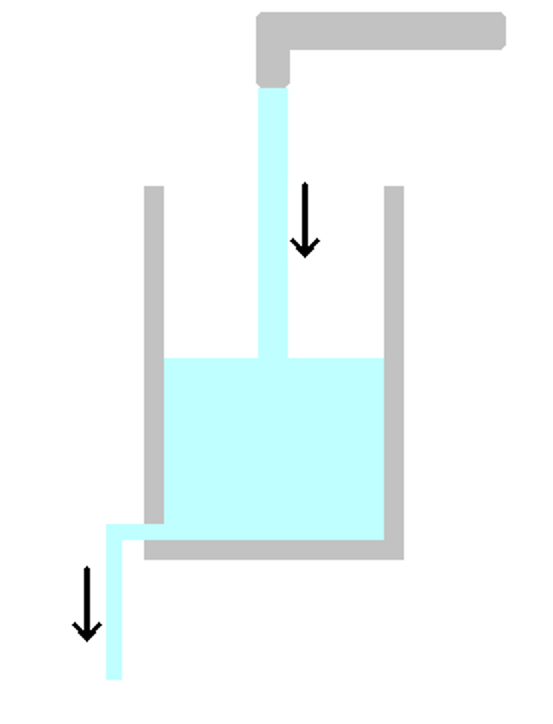
\includegraphics[height=6cm]{glass_tap_up.png}
  \end{center}
  
  
\end{frame}



\begin{frame}{A leaky bucket - increased inflow}

  \begin{center}
    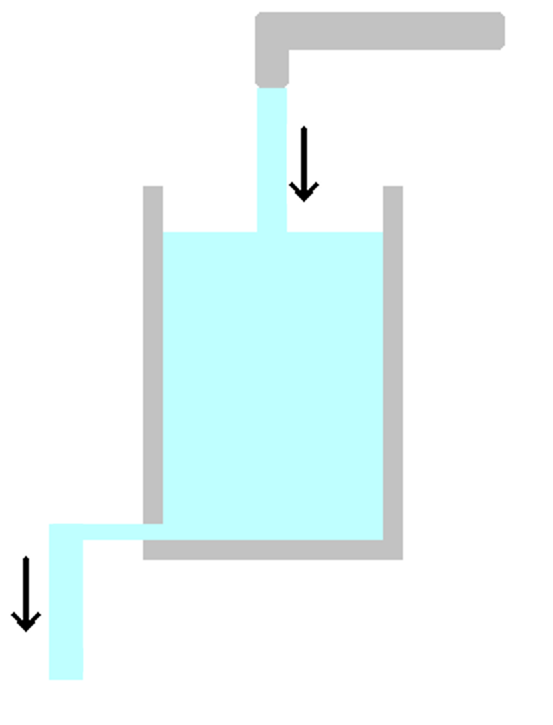
\includegraphics[height=6cm]{glass_level_up.png}
  \end{center}
  
  
\end{frame}



\begin{frame}{A leaky bucket - decreased inflow}

  \begin{center}
    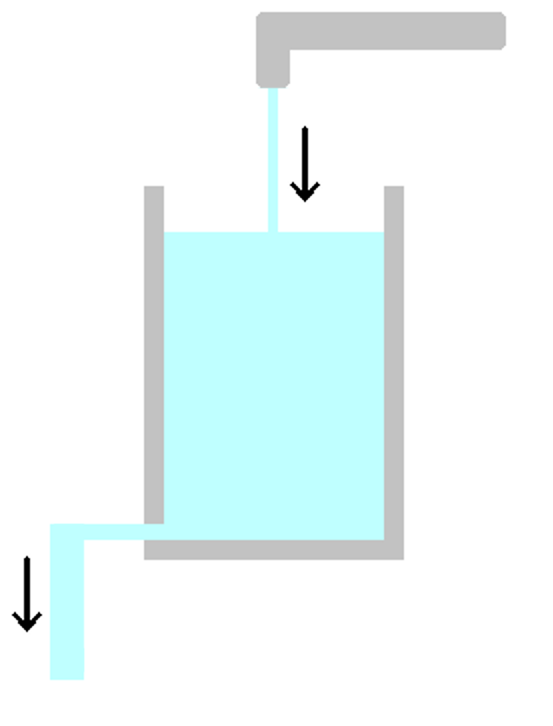
\includegraphics[height=6cm]{glass_tap_down.png}
  \end{center}
  
  
\end{frame}



\begin{frame}{A leaky bucket - decreased inflow}

  \begin{center}
    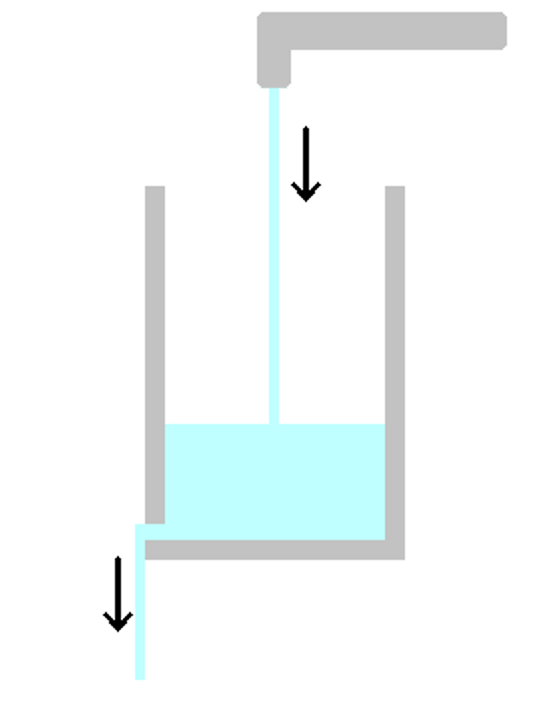
\includegraphics[height=6cm]{glass_level_down.png}
  \end{center}
  
\end{frame}


\begin{frame}{A leaky bucket - notation}
\begin{columns}
\begin{column}{0.5\textwidth}
  \begin{center}
     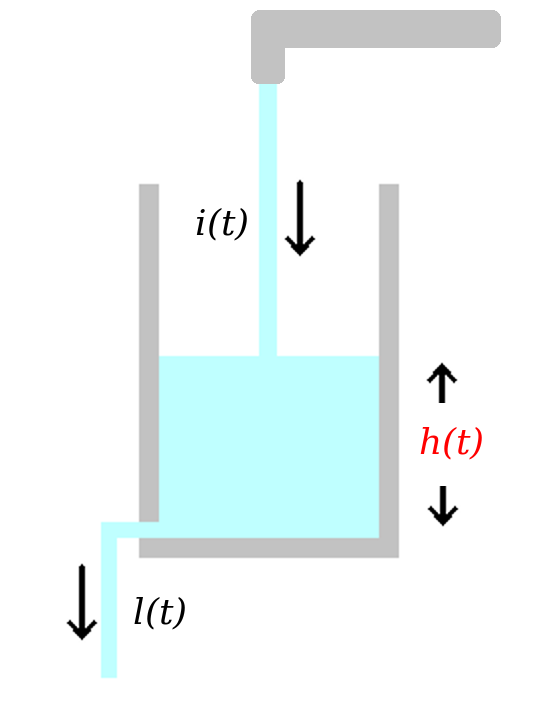
\includegraphics[height=6cm]{glass_h_red.png}      
     \end{center}
\end{column}
\begin{column}{0.5\textwidth}
\cred{} $h(t)$\color{black}{} is the height of the water.
\end{column}
\end{columns}
\end{frame}



\begin{frame}{A leaky bucket - notation}
\begin{columns}
\begin{column}{0.5\textwidth}
  \begin{center}
     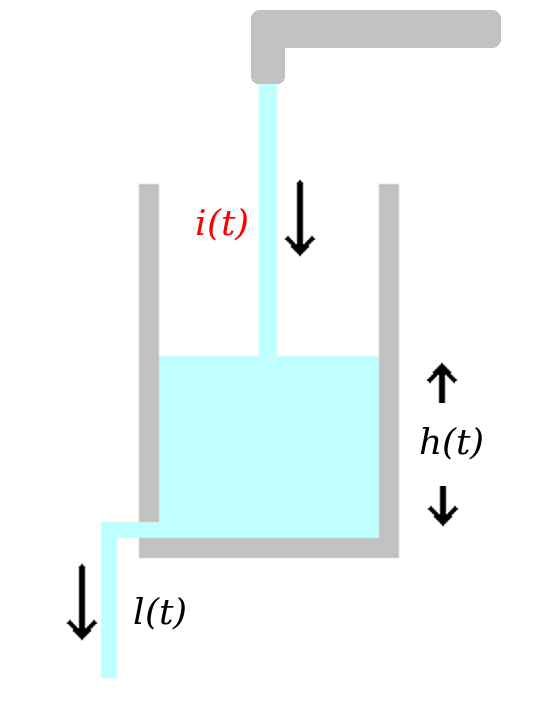
\includegraphics[height=6cm]{glass_i_red.png}      
     \end{center}
\end{column}
\begin{column}{0.5\textwidth}
  \cred{} $i(t)$\color{black}{} is the rate of flow into the
  bucket.\\[1cm] It is a \textsl{rate} so it would be meaured in
  volume per time, for example, \crish$Ls^{-1}$\cbla.
\end{column}
\end{columns}
\end{frame}


\begin{frame}{A leaky bucket - notation}
\begin{columns}
\begin{column}{0.5\textwidth}
  \begin{center}
     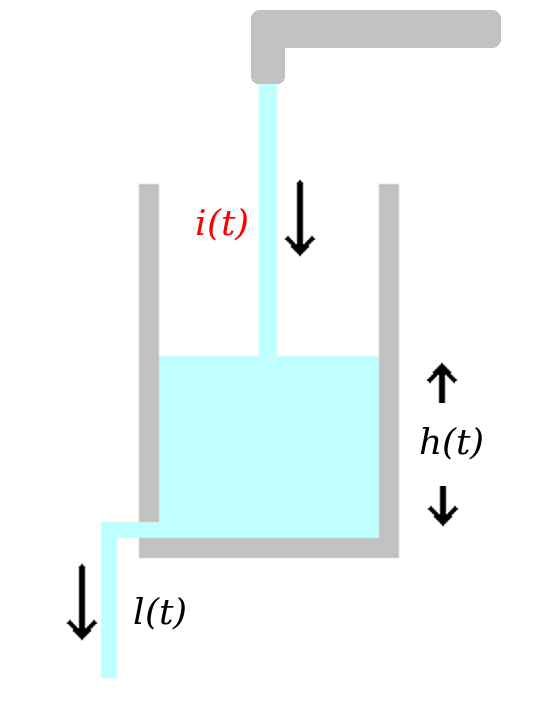
\includegraphics[height=6cm]{glass_i_red.png}      
     \end{center}
\end{column}
\begin{column}{0.5\textwidth}
  \cred{} $l(t)$\color{black}{} is the rate of flow out of the
  bucket.\\[1cm] It is a \textsl{rate} so it would be meaured in
  volume per time, for example, \crish$Ls^{-1}$\cbla.
  
\end{column}
\end{columns}
\end{frame}


\begin{frame}{A leaky bucket - leak}
\begin{columns}
\begin{column}{0.5\textwidth}
  \begin{center}
     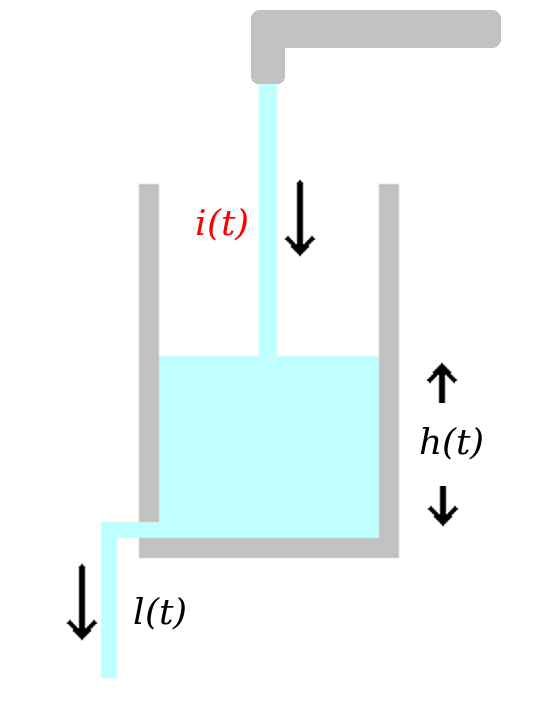
\includegraphics[height=6cm]{glass_i_red.png}      
     \end{center}
\end{column}
\begin{column}{0.5\textwidth}
  The speed of the leak depends on the hieght of the water so\crish
  $$l(t)\propto h(t)$$
  \cbla{}or, adding a constant of proportionality\crish
  $$l(t)=Gh(t)$$
  \cbla{}where \crish{}$G$\cbla{} depends on some physics stuff we aren't interested in here.


  
\end{column}
\end{columns}
\end{frame}


\begin{frame}{A leaky bucket - net flow}
\begin{columns}
\begin{column}{0.5\textwidth}
  \begin{center}
     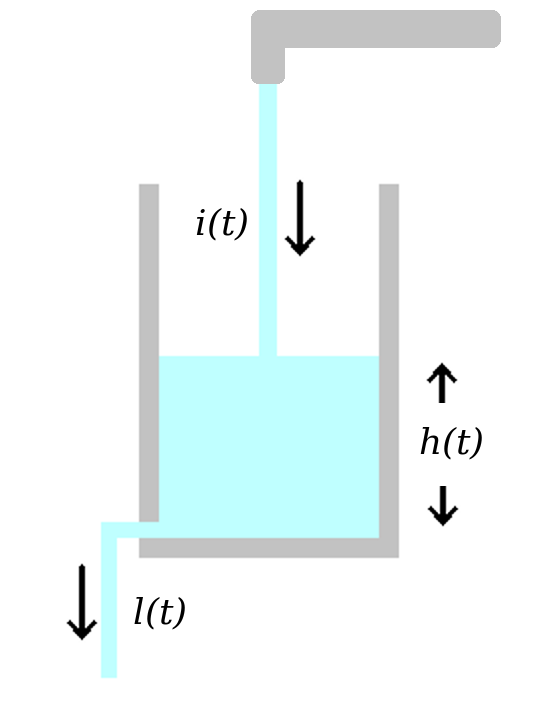
\includegraphics[height=6cm]{glass_notation.png}      
     \end{center}
\end{column}
\begin{column}{0.5\textwidth}
  The net flow into the bucket is therefore\crish
  $$i(t)- l(t)$$
  \cbla{}or,\crish{} 
  $$i(t)-Gh(t)$$
  \cbla{}and, remember this is a flow, so it is measured in volume per time.

\end{column}
\end{columns}
\end{frame}


\begin{frame}{A leaky bucket - volumn}
\begin{columns}
\begin{column}{0.5\textwidth}
  \begin{center}
     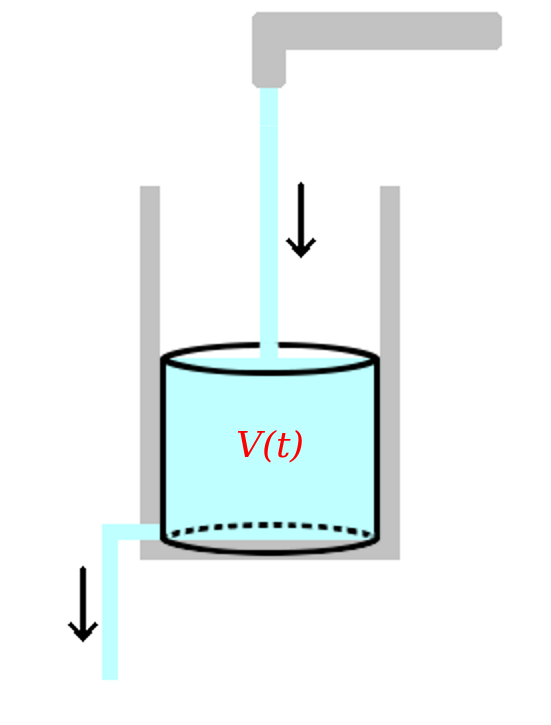
\includegraphics[height=6cm]{glass_volume_notation.png}      
     \end{center}
\end{column}
\begin{column}{0.5\textwidth}
  The net flow changes the volume of water.\\[0.5cm]
  
The volume depends on the height:
  \crish
  $$V(t)=Ch(t)$$ \cbla{}where \crish$C$\cbla{} is a constant.\\[0.5cm]
  In the case of a
  cylindrical bucket, using the formula for the volumn of a cylinder
  tells us that \crish$C=\pi r^2$\cbla{} where \crish$r$\cbla{} is the
  radius of the bucket; but we'll just call it \crish$C$\cbla.
\end{column}
\end{columns}
\end{frame}

\begin{frame}{Equation for a leaky bucket}

  The rate of change of the volume is equal to the net inflow. The
  rate of change is given by the derivative:\crish
  $$\frac{dV}{dt}=i-Gh$$
  \cbla{}
\end{frame}


\begin{frame}{Equation for a leaky bucket}

  The rate of change of the volume is equal to the net inflow. The
  rate of change is given by the derivative:\crish
  $$\frac{dV}{dt}=i-Gh$$
  \cbla{}Notice that when we want to emphasis that something changes with time we write the brackets \crish$t$\cbla, like \crish$h(t)$\cbla{} but at other times we leave it out to stop making equations look to cluttered!\cbla.
\end{frame}


\begin{frame}{Equation for a leaky bucket}
  \crish
  $$\frac{dV}{dt}=i-Gh$$
  \cbla{}Substituting \crish$V=Ch$\cbla{} we get\crish
  $$\frac{d\cblu Ch\crish}{dt}=i-Gh$$
  \cbla{}Since \crish$C$\cbla{} is a constant this means\crish
  $$C\frac{dh}{dt}=i-Gh$$\cbla
  This is our basic equation for the height of the water in a leaky bucket.
\end{frame}


\begin{frame}{Equation for a leaky bucket}
  Let's rewrite this equation as 
  \crish
  $$\cblu\tau\crish\frac{dh}{dt}=\frac{1}{G}i-h$$\cbla where
  \cblu$\tau\crish{}=C/G$\cbla{}.\\[1cm]
  This notation is used because
  \cblu$\tau$\cbla{} is a timescale and \crish$\tau$\cbla{} is the
  Greek equivalent of \crish$t$\cbla. If you work out all the units for the constants \crish$C$\cbla{} and \crish$G$\cbla{} you can see \cblu$\tau$\cbla{} has units of time; it also balances the \textsl{per time} in the derivative. 
\end{frame}

\begin{frame}{Constant input}
  First lets looks at what happens when the water is flowing in at a constant rate, that is when \crish$i$\cbla{} doesn't change with time; lets write\crish{}
  $$i=\bar{\i}$$ when the input is constant.
\end{frame}

\begin{frame}{Behaviour of the equation}
  \crish
  $$\tau\frac{dh}{dt}=\frac{1}{G}\bar{\i}-h$$\cbla If
  \cblu{}$\bar{\i}=Gh$\cbla{} then \cblu{}$dh/dt=0$\cbla{}. This is
  the equilibrium where the inflow is equal to the outflow.
\end{frame}

\begin{frame}{Behaviour of the equation}
  \crish
  $$\tau\frac{dh}{dt}=\frac{1}{G}\bar{\i}-h$$\cbla If
  \cblu{}$\bar{\i}<Gh$\cbla{} then \cblu{}$dh/dt<0$\cbla{} and the
  level of the water falls; so if the water height is too high it
  decreases towards equilibrium.
\end{frame}


\begin{frame}{A leaky bucket - decreased inflow}

  \begin{center}
    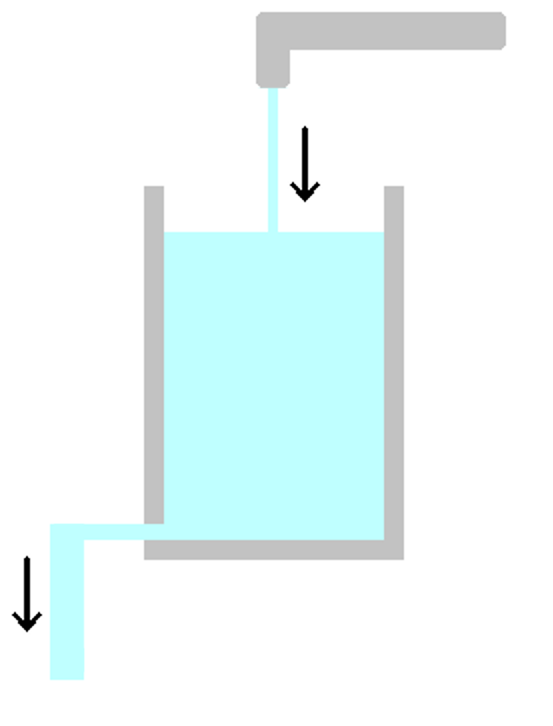
\includegraphics[height=6cm]{glass_tap_down.png}
  \end{center}
  
  
\end{frame}



\begin{frame}{A leaky bucket - decreased inflow}

  \begin{center}
    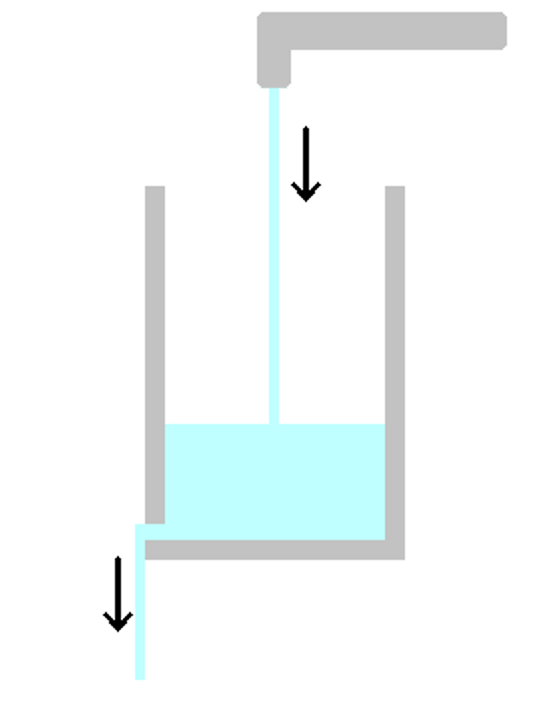
\includegraphics[height=6cm]{glass_level_down.png}
  \end{center}
  
\end{frame}


\begin{frame}{Behaviour of the equation}
  \crish
  $$\tau\frac{dh}{dt}=\frac{1}{G}\bar{\i}-h$$\cbla Conversely if
  \cblu{}$\bar{\i}>Gh$\cbla{} then \cblu{}$dh/dt>0$\cbla{} and the
  level of the water falls; so if the water height is too low it
  increases towards equilibrium.
\end{frame}


\begin{frame}{Behaviour of the equation}
  \crish
  $$\tau\frac{dh}{dt}=\frac{1}{G}\bar{\i}-h$$\cbla Notice also tht the more
  \crish{}$\bar{\i}>Gh$\cbla{} the more \crish{}$dh/dt>0$\cbla{} and \textsl{visa versa} for \crish{}$\bar{\i}<Gh$\cbla: the further the hieght is from the equilibrium, the faster it goes towards equilibrium.
\end{frame}


\end{document}

